\chapter{Les espaces de base}
\begin{abstract}
Dans les problèmes que nous envisageons de traiter \emph{in fine}, il n'est finalement
besoin que d'espaces vectoriels normés finis sur le corps des réels.
On pourrait rapidement en donner les principales propriétés qui sont sans doute encore
en mémoire des lecteurs tant elles sont «naturelles».

Mais en faisant cela, nous ne respecterions pas nos engagements de présenter un
peu plus avant les fondements mathématiques.

Sans toutefois aller trop loin dans les notions topologiques générales, nous allons
essayer dans ce chapitre de passer en revue la liste des espaces depuis les espaces
topologiques jusqu'aux espaces de Hilbert, de manière succincte et didactique (nous
l'espérons) en relevant les points importants essentiellement du point de vue de leur
utilité.
%
%\medskip
%Pour la bibliographie, nous nous référerons comme d'habitude à:\\
%\indent --
%Laurent \textsc{Schwartz}, \emph{Analyse I: Théorie des ensembles et Topologie},
%Hermann, 1992.\\
%%ainsi que:
%\indent --
%Laurent \textsc{Schwartz}, \emph{Analyse III: Calcul intégral}, Hermann, 1992.
\end{abstract}

\section{Panorama non exhaustif des espaces}

\begin{histoire}%
Le mot «topologie» vient de la contraction des noms grecs «topos» (lieu) et «logos» (étude),
c'est donc l'étude du lieu. On a d'ailleurs commencé par l'appeler \emph{Analysis Situs}, le terme
«topologie» n'étant introduit qu'en 1847, en allemand, par Johann Benedict Listing
dans Vorstudien zur Topologie.\index[aut]{Listing (Johann Benedict), 1808-1882, Allemand}

La topologie vise à définir ce qu'est un lieu (i.e. un espace) et quelles peuvent être ses propriétés
(je dirais uniquement en tant que tel, sans autre ajout).
Elle s'intéresse plus précisément à ce que l'on appelle aujourd'hui espaces topologiques et aux
applications, dites continues, qui les lient, ainsi qu'à leurs déformations
(``\emph{A topologist is one who doesn't know the difference between a doughnut and a coffee cup}'').

\sbox{\MaBoiteAvecPhotos}{\setlength{\tabcolsep}{0pt}\scriptsize%
\begin{tabular}{ccc}%
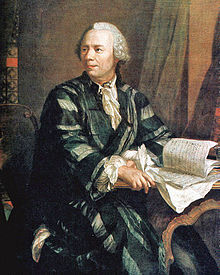
\includegraphics[height=\the\HauteurDesPhotos]{Euler}&%
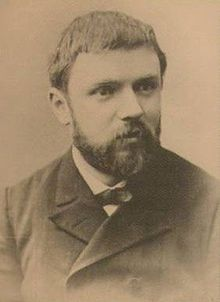
\includegraphics[height=\the\HauteurDesPhotos]{Poincare}&%
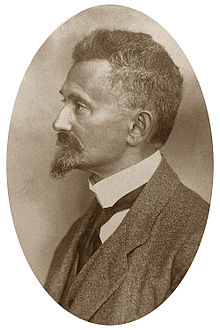
\includegraphics[height=\the\HauteurDesPhotos]{Hausdorff}\\%
Euler&Poincaré&Hausdorff%
\end{tabular}}
\medskip
\ImageADroite{%
En analyse, elle fournit des informations sur l'espace considéré permettant d'obtenir un certain nombre de
résultats (existence et/ou unicité de solutions d'EDP, notamment).
%
Les espaces métriques ainsi que les espaces vectoriels normés sont des exemples d'espaces topologiques.
%
%\medskip
L'origine de la topologie est l'étude de la géométrie dans les cultures antiques.
Le travail de Leonhard Euler\index[aut]{Euler (Leonhard Paul), 1707-1783, Suisse}
datant de 1736 sur le problème des sept ponts de Königsberg est
considéré comme l'un des premiers résultats de géométrie qui ne dépend d'aucune mesure,
i.e. l'un des premiers résultats topologiques.
}

Henri Poincaré\index[aut]{Poincaré (Henri), 1854-1912, Français}
 publia \emph{Analysis Situs} en 1895, introduisant les concepts d'homotopie et d'homologie.
Bien d'autres mathématiciens ont contribué au sujet parmi lesquels nous citerons:
Cantor, Volterra, Arzelà, Hadamard, Ascoli, Fréchet, Hausdorff...\index[aut]{Cantor (Georg Ferdinand Ludwig Philip), 1845-1918, Allemand}\index[aut]{Hadamard (Jacques Salomon), 1865-1963, Français}\index[aut]{Ascoli (Giulio), 1843-1896, Italien}\index[aut]{Fréchet (Maurice René), 1878-1973, Français}\index[aut]{Hausdorff (Felix), 1868-1942, Allemand}

%La notion de métrique s'invite rapidement dans ce chapitre, mais dans ce premier paragraphe,
%nous allons essayer de l'éviter pour n'en parler qu'au paragraphe suivant.
%
Finalement, une dernière généralisation en 1922, par Kuratowski, donna le concept actuel d'espace
topologique.\index[aut]{Kuratowski (Kazimierz), 1896-1980, Polonais}
\end{histoire}
\colorblack


\newpage
\medskip
\subsection{Point de vue topologique}

\begin{marge}
\noindent\tikz[remember picture,baseline] \node[fill=ocre!10,inner sep=3pt](t1) {$E$, un ensemble};

{\small \colorgreen
\noindent
Cela suffit déjà pour pouvoir s'intéresser par exemple à des fonctions, à des relations d'équivalence
(donc au quotient)... décomposition canonique, permutation...

On peut ensuite définir un ensemble ordonné...}

\medskip %\noindent
\textcolorblue{Une topologie}\index{topologie}~$T$ est
un ensemble de parties de~$E$ que l'on définit comme les ouverts de~$(E,T)$, vérifiant les
propriétés suivantes:
\begin{itemize}
  \item L'ensemble vide et~$E$ appartiennent à~$T$.
  \item Toute réunion quelconque d'ouverts est un ouvert, i.e. si~$(O_i)_{i\in I}$ est une famille
	d'éléments de~$T$, indexée par un ensemble~$I$ quelconque (pas nécessairement fini ni
	même dénombrable) alors~$\bigcup_{i \in I}O_i \in T$.
  \item Toute intersection finie d'ouverts est un ouvert, i.e. si~$O_1, ..., O_n$ sont des éléments de~$T$
	(avec~$n > 0$), alors~$O_1\cap \ldots \cap O_n \in T$.
\end{itemize}



\noindent\tikz[remember picture,baseline] \node[fill=ocre!10,inner sep=3pt](t2) {Espace topologique};\index{espace!topologique}

{\small \colorgreen\noindent
À partir des ouverts, on définit les fermés, l'adhérence, l'intérieur,
l'extérieur, voisinage...
}

\medskip
\textcolorblue{Séparation}: % (dit aussi «axiome~$T_2$» au sein des axiomes de séparation):

deux points distincts quelconques admettent toujours des voisinages disjoints.



\noindent\tikz[remember picture,baseline] \node[fill=ocre!10,inner sep=3pt](t3) {Espace séparé (ou de Hausdorff)};
\index{espace!séparé}\index{espace!de Hausdorff}\index[aut]{Hausdorff (Felix), 1868-1942, Allemand}

{\small \colorgreen
\noindent Intérêts:
\begin{itemize}
  \item Unicité de la limite de tout filtre convergent.
  \item Une suite convergente a une limite unique.
  \item Une topologie plus fine qu'une topologie séparée est séparée.
  \item Tout sous-espace d'un espace séparé est séparé.
  \item Deux applications continues à valeurs dans un séparé qui coïncident sur une partie dense sont égales.
\end{itemize}
}

\medskip
\textcolorblue{Régularité}:

Il est possible de séparer un point~$x$ et un fermé~$F$ ne contenant pas~$x$ par deux ouverts disjoints.

On peut même alors choisir ces deux ouverts de manière à ce que leurs adhérences respectives soient disjointes.



\noindent\tikz[remember picture,baseline] \node[fill=ocre!10,inner sep=3pt] (t4) {Espace régulier};\index{espace!régulier}

{\small \colorgreen
\noindent Application:
\begin{itemize}
  \item Tout point admet une base de voisinages fermés.
  \item Tout fermé est l'intersection de ses voisinages fermés.
\end{itemize}
}

\medskip
\textcolorblue{Compacité} (recouvrement fini):\index{compacité}

Un espace séparé est compact (vérifie la propriété de Borel-Lebesgue),
si chaque fois qu'il est recouvert par des ouverts, il est recouvert par un nombre fini d'entre eux.



\noindent\tikz[remember picture,baseline] \node[fill=ocre!10,inner sep=3pt] (t5) {Espace compact};\index{espace!compact}

{\small \colorgreen
Tout produit de compacts est compact.

$\overline{\RR}$ est compact

Un espace peut ne pas être compact, mais une de ses parties l'être:
\begin{itemize}
  \item~$\RR$ n'est pas fermé, mais tout~$[a;b]$ fermé borné l'est.
  \item~$\RR^n$ n'est pas compact, mais tout pavé fermé l'est.
\end{itemize}
}
\begin{tikzpicture}[remember picture,overlay]
  \draw[->,thick,ocre] (t1.west) -- +(-10pt,0) |-([yshift=2pt]t2.west);
  \draw[->,thick,ocre] ([yshift=-2pt]t2.west) -- +(-10pt,0) |-([yshift=2pt]t3.west);
  \draw[->,thick,ocre] ([yshift=-2pt]t3.west) -- +(-10pt,0) |-([yshift=2pt]t4.west);
  \draw[->,thick,ocre] ([yshift=-2pt]t4.west) -- +(-10pt,0) |-(t5.west);
\end{tikzpicture}
\end{marge}

\medskip
\textcolorred{Notons bien que rien n'est dit sur les éléments de l'ensemble~$E$.
Ce peuvent être des éléments discrets, des scalaires, des vecteurs,
des fonctions...}

%\medskip
\newpage
\subsection{Point de vue métrique}
Comme nous le mentionnions au paragraphe précédent, lorsque l'on parle d'espace
on a intuitivement envie de parler de «distance».

%\medskip
\begin{histoire}
Unifiant les travaux de ses prédécesseurs sur les espaces de fonctions, c'est en 1906 que
Maurice Fréchet introduit le concept d'espace métrique.\index[aut]{Fréchet (Maurice René), 1878-1973, Français}

\sbox{\MaBoiteAvecPhotos}{\setlength{\tabcolsep}{0pt}\scriptsize%
\begin{tabular}{cc}%
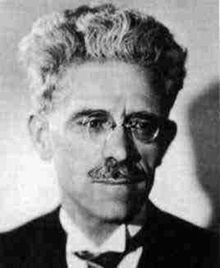
\includegraphics[height=\the\HauteurDesPhotos]{Frechet}&%
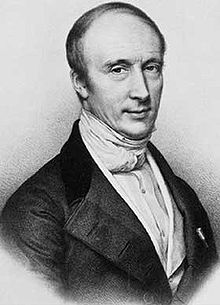
\includegraphics[height=\the\HauteurDesPhotos]{Cauchy}\\%
Fréchet&Cauchy
\end{tabular}}
\medskip
\ImageADroite{%
La métrique qui nous est la plus usuelle est évidemment la métrique euclidienne,\index[aut]{Euclide, -325-- -265, Grec}
qui est celle que nous utilisons en géométrique «classique» (euclidienne):
la distance entre deux points est égale à la longueur du segment les reliant.
La structure métrique fournit beaucoup plus d'information sur la forme géométrique
des objets que la structure topologique.\\
\indent
Enfin nous redonnerons le si important critère de Cauchy\index[aut]{Cauchy (Augustin Louis, baron -), 1789-1857, Français}
(qui est valable %non seulement pour les réels, aussi également pour les complexes, et d'une manière encore plus générale
pour tout espace uniforme, dont notamment les espaces métriques) qui permet de définir la toute aussi importante notion
de complétude.
}
%Ce critère est vérifié par une suite lorsque les termes de celle-ci se «rapprochent uniformément les uns des autres en l'infini\fg.
%Elle est alors celles susceptible de converger.
%Le critère de Cauchy ne sera présenté que dans le cas des espaces métriques.
\end{histoire}
\colorblack

\medskip
\begin{marge}%
\noindent\tikz[remember picture,baseline] \node[fill=ocre!10,inner sep=3pt] (n1) {$E$, un ensemble};

Une \textcolorblue{distance ou métrique}~$d$\index{distance}\index{métrique}
est une application de~$E\times E \rightarrow \RR_+$ telle que:
\begin{itemize}
  \item~$d(x,y)=d(y,x)$ (symétrie);
  \item~$d(x,y)>0$ si~$x\ne y$, et~$d(x,x)=0$ (positivité);
  \item~$d(x,z)\le d(x,y)+d(y,z)$ (inégalité triangulaire).
\end{itemize}



\noindent\tikz[remember picture,baseline] \node[fill=ocre!10,inner sep=3pt] (n2) {Espace métrique\index{espace!métrique}};

{\small \colorgreen\noindent
On peut réexprimer les notions d'ouvert, fermé, adhérence... densité, continuité... avec la métrique
(les~$\varepsilon$...).

\noindent Deux normes sont équivalentes si elles définissent la même topologie.

\noindent Deux normes~$\|\cdot\|_1$ et~$\|\cdot\|_2$ sont équivalentes s'il existe deux constantes strictement positives~$k'$ et~$k''$ telles que $\forall x\in E$, $\|x\|_1\le k'\|x\|_1$ et $\|x\|_2\le k'' \|x\|_1$.}

\medskip
\textcolorblue{Critère de Cauchy:}\index{critère de Cauchy}\index[aut]{Cauchy (Augustin Louis, baron -), 1789-1857, Français}

Soit~$E$ un espace métrique et soit~$x_0$, $x_1$, ..., $x_n$, ...
une suite d'éléments de~$E$.
Cette suite est de Cauchy de~$E$ si:
\begin{equation}
\forall\varepsilon>0, \exists N\in\NN, (\forall n\in\NN, \forall m\in\NN,
n\ge N, m\ge N): d(x_m,x_n)\le\varepsilon
\end{equation}
ou encore:~$d(x_m,x_n)$ tend vers~$0$ quand~$m$ et~$n$ tendent
vers l'infini.



\noindent \tikz[remember picture,baseline] \node[fill=ocre!10,inner sep=3pt] (n3) {Espace métrique complet\index{espace!métrique!complet}};

{\small \colorgreen\noindent
Toute suite convergente est de Cauchy.

\noindent Réciproque: si~$x_0$, $x_1$, ..., $x_n$, ... est de Cauchy sur
$\RR$ ou~$\CC$, alors elle converge.
}

\medskip\noindent
\textcolorred{Cette propriété est fondamentale car elle permet de reconnaître si une suite
converge sans connaître sa limite.}
%Mais attention, ce n'est pas vrai quelque soit l'espace métrique, mais sur~$\RR$
%et~$\CC$.

\medskip\noindent
Attention, la notion d'espace complet est une notion métrique et non topologique
(elle peut donc être vraie pour une métrique et fausse pour une autre).

\medskip\noindent
\textcolorred{L'importance de la complétude} tient à ce que la solution d'un problème passe souvent
par une solution approchée. Si la suite des solutions approchées est de Cauchy d'un espace convenable,
et si cet espace est complet, alors la convergence vers une solution du problème est assurée.
\begin{tikzpicture}[remember picture,overlay]
  \draw[->,thick,ocre] (n1.west) -- +(-10pt,0) |-([yshift=2pt]n2.west);
  \draw[->,thick,ocre] ([yshift=-2pt]n2.west) -- +(-10pt,0) |-(n3.west);
\end{tikzpicture}
\end{marge}

\medskip
\subsection{Point de vue algébrique}

\medskip
Jusqu'à présent, nous n'avons pas vraiment parlé d'opérations que nous
pourrions effectuer à l'intérieur des espaces que nous avons définis, ou entre
ces espaces.
%
\textcolorgris{\small Pour une présentation des structures algébriques on se reportera au cours homonyme.
Elles sont riches et nombreuses.
Dans le cadre de ce document, nous ne nous intéresserons qu'au cas de la structure
d'espace vectoriel, le but étant, comme mentionné en introduction, d'en arriver aux
espaces de Hilbert, fondements de l'analyse fonctionnelle.}

\medskip
\begin{histoire}
Lorsque l'on demande de citer l'un des grands mathématiciens du \textsc{xx}\fup{e} siècle,
Henri Poincaré\index[aut]{Poincaré (Henri), 1854-1912, Français}
et David Hilbert\index[aut]{Hilbert (David), 1862-1943, Allemand}
se partagent souvent la première place, aussi
bien pour l'éventail considérable des sujets qu'ils ont
abordés que pour avoir fait émerger de nombreuses idées fondamentales.

\sbox{\MaBoiteAvecPhotos}{\setlength{\tabcolsep}{0pt}\scriptsize%
\begin{tabular}{cc}%
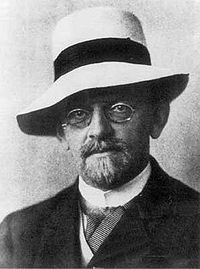
\includegraphics[height=\the\HauteurDesPhotos]{Hilbert}&%
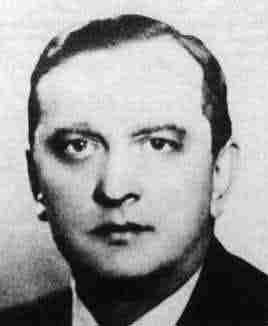
\includegraphics[height=\the\HauteurDesPhotos]{Banach}\\%
Hilbert&Banach%
\end{tabular}}
\medskip
\ImageADroite{%
Hilbert reste célèbre pour ses 23 problèmes (dits problèmes de Hilbert)
qu'il présenta au deuxième congrès international des mathématiciens à Paris en 1900,
qui tenaient jusqu'alors les mathématiciens en échec et devaient marquer le cours
des mathématiques du \textsc{xx}\fup{e} siècle (et il avait raison; tous ne sont pas résolus à ce jour).\\
\indent
Nous croiserons également un autre fondateur de l'analyse fonctionnelle, Stephan Banach
\index[aut]{Banach (Stephan), 1892-1945, Polonais}
qui a généralisé entre autre les travaux de Hilbert sur les équations intégrales,
notamment en approfondissant la théorie des espaces vectoriels topologiques.
}
\end{histoire}
\colorblack





\medskip
\begin{marge}
\noindent\tikz[remember picture,baseline] \node[fill=ocre!10,inner sep=3pt] (b1) {$E$, un ensemble};


\medskip
\textcolorblue{Structure d'espace vectoriel}:

C'est une structure comportant une loi de composition interne et une loi de composition externe sur un corps~$\KK$ permettant d'effectuer des combinaisons
linéaires (voir cours sur les structures algébriques).

La loi de composition interne, notée~$+$ en fait un groupe abélien, la loi de composition externe est la multiplication par un scalaire,
scalaire pris sur le corps~$\KK$ considéré.

\noindent\tikz[remember picture,baseline] \node[fill=ocre!10,inner sep=3pt] (b2) {Espace vectoriel (topologique)\index{espace!vectoriel!topologique}};

{\small \colorgreen\noindent
Sur un espace vectoriel de dimension finie sur~$\RR$ ou~$\CC$, 2 normes quelconques sont
équivalentes.}

\medskip
Une \textcolorblue{norme sur un espace vectoriel}~$E$\index{norme}
est une fonction, $x \mapsto \|x\|$ possédant les propriétés:
\begin{itemize}
  \item positivité:~$\|x\|>0$ pour~$x\ne0$, $\|0\|=0$;
  \item transformation par les homothéties:~$\|\lambda x\|=|\lambda|\| x\|, \lambda\in\KK$;
  \item inégalité de convexité:~$\|x+y\|\le\|x\|+\|y\|$.
\end{itemize}

La \textcolorblue{distance issue de la norme} est la distance définie par~$d(x,y)=\|x-y\|$.

\noindent\tikz[remember picture,baseline] \node[fill=ocre!10,inner sep=3pt] (b3) {Espace vectoriel normé\index{espace!vectoriel!normé}};

{\small \colorgreen\noindent
Tout espace vectoriel normé est automatiquement un espace métrique (avec la distance
issue de sa norme).\index{distance!issue d'une norme}
%
%\noindent
De plus:
\begin{itemize}
  \item la distance est invariante par translation:~$d(x-a,y-a)=d(x,y)$.
  \item une homothétie de rapport~$\lambda$ multiplie la distance par~$|\lambda|$:~$d(\lambda x,\lambda y)=|\lambda| d(x,y)$.
\end{itemize}

\noindent Tout espace vectoriel normé de dimension finie est localement compact
(i.e. tout point possède au moins un voisinage compact), car toute boule
fermée est compacte.
}

\medskip
Comme un espace vectoriel normé muni avec la distance
issue de sa norme est un espace métrique, on peut se demander si
cet espace métrique vérifie le \textcolorblue{critère de Cauchy}
(voir paragraphe précédent) afin d'en faire un espace complet.

\noindent\tikz[remember picture,baseline] \node[fill=ocre!10,inner sep=3pt](b4) {Espace de Banach\index{espace!de Banach}\index[aut]{Banach (Stephan), 1892-1945, Polonais}};
\begin{tikzpicture}[remember picture,overlay]
  \draw[->,thick,ocre] (b1.west) -- +(-10pt,0) |-([yshift=2pt]b2.west);
  \draw[->,thick,ocre] ([yshift=-2pt]b2.west) -- +(-10pt,0) |-([yshift=2pt]b3.west);
  \draw[->,thick,ocre] ([yshift=-2pt]b3.west) -- +(-10pt,0) |-([yshift=2pt]b4.west);
\end{tikzpicture}


{\small \colorgreen\noindent
C'est donc finalement un espace vectoriel normé sur un sous-corps
$\KK$ de~$\CC$ (en général, $\KK=\RR$ ou~$\CC$), complet pour la distance issue de sa norme.

\noindent Comme la topologie induite par sa distance est compatible avec sa structure d'espace vectoriel,
c'est un espace vectoriel topologique.
}

\medskip
Une norme~$\|\cdot\|$ \textcolorblue{découle d'un produit scalaire ou hermitien}\index[aut]{Hermite (Charles), 1822-1901, Français}\index{produit scalaire}
$\langle\cdot,\cdot\rangle$ si l'on a:~$\| x\| = \sqrt{\langle x,x \rangle}$.%footnote

\noindent\tikz[remember picture,baseline] \node[fill=ocre!10,inner sep=3pt](b5) {Espace de Hilbert\index{espace!de Hilbert}\index[aut]{Hilbert (David), 1862-1943, Allemand}};
\begin{tikzpicture}[remember picture,overlay]
  \draw[->,thick,ocre] ([yshift=-2pt]b4.west) -- +(-10pt,0) |-(b5.west);
\end{tikzpicture}


{ \small \colorgreen\noindent
C'est donc un espace préhilbertien complet, i.e.
un espace de Banach dont la norme découle d'un produit scalaire ou hermitien\index[aut]{Hermite (Charles), 1822-1901, Français} \textcolorred{unique}.

\noindent Un espace de Hilbert est la généralisation en dimension quelconque d'un espace euclidien\index[aut]{Euclide, -325-- -265, Grec}
	ou hermitien\index[aut]{Hermite (Charles), 1822-1901, Français}
	(Un \textbf{espace vectoriel euclidien} est un espace vectoriel réel de dimension finie muni d'un produit scalaire).

}
\end{marge}

\medskip
On peut encore faire les remarques suivantes concernant les espaces de Hilbert:
\begin{itemize}
  \item Tout sous-espace vectoriel fermé d'un Hilbert est un Hilbert.
  \item \textcolorred{Le plus important} est de disposer d'un produit scalaire, car on va alors pouvoir déterminer des parties
	orthogonales de l'espace, donc en somme directe (théorème~\ref{th:projHilbert}).

	On rappelle, si besoin, qu'un \textcolorblue{produit scalaire}\index{produit scalaire} est une
	forme bilinéaire\index{forme!bilinéaire} (i.e. une application\index{application} de~$E\times E$
	dans~$\RR$, linéaire pour chacune des deux variables) possédant les propriétés:
	\begin{itemize}
	  \item symétrie:~$\forall x,y \in E$, $\langle x\, , \, y \rangle = \langle y\, , \, x\rangle$
	  \item positivité:~$\forall x \in E$, $\langle x\, , \, x \rangle \; \ge \; 0$
	  \item définie:~$\forall x \in E$, $\big(\ \langle x\, , \, x \rangle = 0 \; \Rightarrow x = 0\ \big)$
	\end{itemize}
	ce qui se traduit pas la définition: «Un produit scalaire sur un espace vectoriel réel~$E$ est une
	forme bilinéaire symétrique définie positive».
\end{itemize}


\medskip
Quelques espaces de Banach:
\begin{itemize}
\item Les espaces euclidiens\index[aut]{Euclide, -325-- -265, Grec}~$\RR^n$ et
les espaces hermitiens\index[aut]{Hermite (Charles), 1822-1901, Français}~$\CC^n$
munis de la norme:
\begin{equation}\|(x_1,\ldots,x_n)\| = \sqrt{\dsum_{i=1}^n x_i \overline{x_i}}\end{equation} où~$\overline{x_i}$
désigne le conjugué de~$x_i$.

\item L'espace des fonctions (dans~$\RR$ ou~$\CC$) continues et bornées sur un espace topologique~$X$,
muni de la norme~$\|f\| = \sup_{x \in X}(|f(x)|)$.
En particulier, l'espace des fonctions continues sur un espace~$X$ compact, comme un intervalle réel~$\intff{a}{b}$.

\item Pour tout réel~$p \ge 1$, l'espace~$L^p$ des classes de fonctions mesurables, dans~$\RR$ ou~$\CC$, sur un espace mesuré~$X$.
\end{itemize}

\medskip
Quelques espaces de Hilbert:
\begin{itemize}
  \item Certains espaces de Sobolev (voir plus loin) sont des espaces de Hilbert (ceux qui nous intéresserons
en général, ça tombe bien).
  \item L'espace euclidien\index[aut]{Euclide, -325-- -265, Grec}~$\RR^n$ muni du produit scalaire
usuel est hilbertien,\index[aut]{Hilbert (David), 1862-1943, Allemand} ainsi que l'espace~$L^2$.
\end{itemize}


\begin{theoreme}[Théorème de complétion sur un espace de Banach]\label{th:complbanach}\index{théorème!de complétion (sur un Banach)}
Soit~$E$ un espace vectoriel normé incomplet.
Alors~$E$ est isomorphe, en tant qu'espace vectoriel, et isométrique à un sous-espace
vectoriel dense dans un espace de Banach~$\overline{E}$.

Cet espace de Banach~$\overline{E}$ est unique à un isomorphisme isométrique près.
\end{theoreme}

Ce théorème de complétion répond par l'affirmative à la question:
si l'espace normé~$E$ n'est pas complet, existe-t-il un Banach minimal~$\overline{E}$ le
contenant ?

\begin{theoreme}[Théorème de projection dans un espace de Hilbert]\label{th:projHilbert}\index{théorème!de projection (dans un Hilbert)}
Soit~$F$ un sous-espace vectoriel fermé d'un Hilbert~$H$ (il est alors lui-même un Hilbert).
Alors:
\begin{itemize}
  \item son orthogonal~$F^\bot$, qui est l'ensemble des vecteurs orthogonaux à chaque
	vecteur de~$F$, est un sous-espace vectoriel fermé (donc un Hilbert);
  \item Tout~$h\in H$ s'écrit de façon unique~$h=h'+h''$ où~$h'$ est le projeté
	orthogonal de~$h$ sur~$F$, et~$h''$ le projeté orthogonal de~$h$ sur~$F^\bot$.
\end{itemize}
\end{theoreme}

%\medskip
Les points importants de ce théorème de projection sont que cette décomposition est
unique, et que l'on a~$H=F\oplus F^\bot$ (on parle parfois de «somme hilbertienne»).


%\medskip
\section{Tribu, mesure, espaces mesurable et mesuré}

En complément à l'aspect métrique (Fréchet 1906), nous
\index[aut]{Fréchet (Maurice René), 1878-1973, Français}
allons maintenant aborder l'aspect mesure.

\medskip
Le but, à travers la notion de mesure, est d'étendre la notion usuelle de longueur pour les ensembles
de~$\RR$, ou de volume pour ceux de~$\RR^n$, et ceci de deux manières:
\begin{itemize}
\item on veut d'une part pouvoir considérer des espaces de base plus généraux (plus «abstraits»:
espaces de dimension infinie, espaces sur lesquels on définit les probabilités...); 
\item et
d'autre part on veut englober dans le même cadre mathématique les notions de longueurs, 
surface, volume, mais aussi de masses ou charges ponctuelles issues de la mécanique, de
l'électricité... car toutes ces quantités possèdent une même propriété évidente: l'\textcolorblue{additivité}
(i.e. si l'on désigne par~$\mu(A)$ le volume, la masse, la charge électrique... d'une partie «raisonnable»~$A$,
alors~$\mu(A\cap B)=\mu(A)+\mu(B)$ dès que~$A$ et~$B$ sont disjoints).
\end{itemize}

\medskip
Afin de réaliser cela, il faut en passer par quelques complications mathématiques, et cela essentiellement
pour deux raisons.
Il nous faut tout d'abord définir ce qu'est une partie «raisonnable» d'un ensemble~$E$ (s'il est
aisé de définir le volume d'un polyèdre par exemple, il existe des parties dont la «frontière» est
si complexe qu'elles ne possèdent pas de notion de volume).
Ensuite, la propriété d'additivité si dessus est un peu trop naïve et se révèle insuffisante pour avoir de bonnes 
propriétés pour les mesures.

En effet, la classe des mesures additives a une structure mathématique extrêmement pauvre, ne permettant pas, 
en particulier, de définir une notion satisfaisante d'intégrale par rapport à ces mesures additives.
On est donc conduit à utiliser les mesures possédant la propriété de~$\sigma$-additivité (voir définition
d'une mesure ci-dessous), ce qui nous oblige à considérer comme classe d'ensembles «mesurables» une 
tribu (voir définition de tribu ci-dessous) au lieu de la notion plus simple d'algèbre.

\medskip
\begin{definition}[Algèbre]
Une \textcolorblue{algèbre (de Boole)\index[aut]{Boole (George), 1815-1864, Anglais}~$\mathcal{E}$} sur un ensemble 
$X$ est un \textcolorred{ensemble} non vide de parties de~$X$, stable par passage au complémentaire et par union finie
(donc aussi par intersection finie), i.e.:
\begin{enumerate}
 \item~$\mathcal{E} \not=\varnothing$
 \item~$\forall A \in \mathcal{E}$, ${}^c A \in\mathcal{E}$, où~${}^cA$ désigne le complémentaire de~$A$ dans~$X$.
	(donc~$X\in \mathcal{A}$)
\item si~$A_1,\ldots,A_n$~$\in\mathcal{E}$ alors~$A_1\cup ...\cup A_n \in\mathcal{E}$
\end{enumerate}
\end{definition}

\medskip
\begin{definition}[Tribu]
Une \textcolorblue{tribu~$\mathcal{A}$}\index{tribu} sur un ensemble~$X$ est un \textcolorred{ensemble}
non vide de parties de~$X$, stable par passage au complémentaire et par union dénombrable
(donc aussi par intersection dénombrable), i.e.:
\begin{enumerate}
 \item~$\mathcal{A} \not=\varnothing$
 \item~$\forall A \in \mathcal{A}$, ${}^c A \in\mathcal{A}$%, où~${}^cA$ désigne le complémentaire de~$A$ dans~$X$. (donc~$X\in \mathcal{A}$)
\item si~$\forall n \in \mathbb{N}$, $A_n \in\mathcal{A}$ alors~$\bigcup_{n\in\mathbb{N}} A_n \in\mathcal{A}$
\end{enumerate}
\end{definition}

Ces deux dernières définitions étant placées l'une sous l'autre, leur différence doit apparaître clairement:
dans le cas d'une algèbre, on a à faire à un nombre fini d'intersection ou de réunions, dans celui
d'une tribu, on prend en compte un ensemble dénombrable (donc fini ou non).

\medskip
Il est donc évident que toute tribu est une algèbre, la réciproque étant fausse.

%\medskip
\begin{definition}[Espace mesurable]
Le couple \textcolorblue{$(X,\mathcal{A})$} est appelé \textcolorblue{espace
mesurable}\index{espace!mesurable (probabilisable)} ou espace probabilisable en fonction du contexte.
Sur les espaces mesurables on définit des mesures (voir ci-après); sur les espaces probabilisables, on
appelle ces mesures des probabilités.
\end{definition}

\medskip
\begin{histoire}
La théorie de la mesure s'occupe de regarder un peu plus en détail ce qui se
passe à l'intérieur des espaces dits mesurés (définis plus bas): il s'agit
de mesurer les différentes parties existant dans un tel espace, parties en lien
avec la topologie, ce qui reboucle le sujet...

\medskip
Lorsque l'on évoque le concept de mesure, on en arrive assez rapidement
à se demander: Est-ce que l'on peut tout mesurer? Est-ce
que l'on doit tout mesurer? Qu'est-ce qui est négligeable ?

\sbox{\MaBoiteAvecPhotos}{\setlength{\tabcolsep}{0pt}\scriptsize%
\begin{tabular}{ccc}%
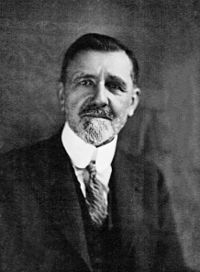
\includegraphics[height=\the\HauteurDesPhotos]{Borel}&%
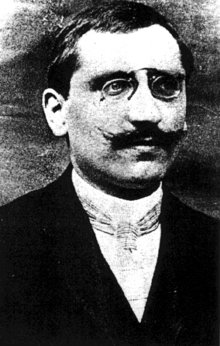
\includegraphics[height=\the\HauteurDesPhotos]{Lebesgue}&%
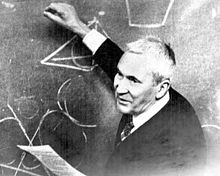
\includegraphics[height=\the\HauteurDesPhotos]{Kolmogorov}\\%
Borel &Lebesgue &Kolmogorov%
\end{tabular}}
\medskip
\ImageADroite{%
En 1894, Émile Borel\index[aut]{Borel (Félix Édouard Justin Émile), 1871-1956, Français} énonce la première définition d'ensemble négligeable.
En 1897, il définit les ensembles mesurables.
En 1901, Henri-Léon Lebesgue\index[aut]{Lebesgue (Henri-Léon), 1875-1941, Français}
 introduit la notion de mesure.
La théorie se développe jusque dans les années 1950.\\\indent
Andreï Kolmogorov\index[aut]{Kolmogorov (Andreï Nikolaïevitch), 1903-1987, Russe}
 proposera une axiomatisation du calcul des probabilités basée notamment
sur l'intégrale définie à partir d'une mesure.
}
\end{histoire}

%\medskip
Les parties de~$X$ qui appartiennent à la tribu~$\mathcal{A}$ sont appelées \textcolorblue{ensembles
mesurables}.\index{ensemble mesurable}
Dans un contexte probabiliste, on les appelle événements (il suffit que~$\mu(X)=1$ pour que~$\mu$ soit
une probabilité).

%\medskip
Une \textcolorblue{mesure~$\mu$}\index{mesure} sur un ensemble~$X$ est une fonction qui
associe à chaque élément d'une tribu d'un ensemble~$X$ un \textcolorred{scalaire positif}
(une longueur, un volume, une probabilité...).

\begin{definition}[Mesure]
\medskip
Soit~$(X,\mathcal{A})$, un espace mesurable.
Une application~$\mu$ définie sur~$\mathcal{A}$, à valeurs dans~$[0,+\infty]$ est appelée
mesure lorsque les deux propriétés suivantes sont satisfaites:
\begin{enumerate}
  \item L'ensemble vide a une mesure nulle:~$\mu\left(\varnothing\right)=0$
  \item L'application~$\mu$ est~$\sigma$-additive:
si~$E_1$, $E_2$, ... est une famille dénombrable de parties de~$X$ appartenant à
$\mathcal{A}$ et si ces parties sont deux à deux disjointes, alors la mesure~$\mu(E)$ de leur réunion
$E$ est égale à la somme des mesures des parties:
\begin{equation}
\mu\left(\bigcup_{k=1}^{\infty}E_{k}\right)=\sum_{k=1}^{\infty}\mu(E_{k}).1
\end{equation}
\end{enumerate}
\end{definition}

On appelle \textcolorblue{espace mesuré un triplet~$(X,\mathcal{A},\mu)$},
\index{espace!mesuré} où~$X$ est un ensemble, $\mathcal{A}$ une tribu sur
$X$ et~$\mu$ une mesure sur~$\mathcal{A}$.

\medskip
\colorgris
Soient~$(X,T)$ et~$(Y,U)$ deux espaces mesurables.
On appelle rectangle mesurable du produit~$\Omega=X\times Y$, toute partie de~$\Omega$
de la forme~$A\times B$ où~$A$ et~$B$ sont des éléments resp de~$T$ et~$U$-mesurables.

On appelle produit tensoriel des deux tribus~$T$ et~$U$, la tribu
engendrée par l'ensemble des rectangles mesurables.
Cette tribu est notée~$T \otimes U$, et est la plus petite tribu de~$\Omega$ qui contient
toutes les parties de la forme~$A\times B$, $A\in T$, $B\in U$.

Le produit des espaces mesurables est~$(X\times Y, T \otimes U)$ et est un espace mesurable:
\begin{equation}
\dint f\,\dd(\mu \otimes \nu) = \dint\dint f(x,y) \dd\mu(x)\dd\nu(y)
\end{equation}
\colorblack

\medskip
\section{Tribu borélienne, mesures de Dirac et Lebesgue}

\begin{definition}[Tribu borélienne]
On appelle \textcolorblue{tribu borélienne}\index{tribu!borélienne} sur un espace topologique donné la tribu engendrée par les
ensembles ouverts.
Dans le cas simple et fondamental de l'espace usuel à~$n$ dimensions, la tribu borélienne de~$\RR^n$
est engendrée par une famille dénombrable de parties, les pavés dont les sommets sont à
coordonnées rationnelles.
\end{definition}

%\medskip
On aura besoin de ces notions (dont la tribu borélienne) pour l'intégrale de Lebesgue et par extension
toute la théorie de l'intégration qui est à la base de l'analyse numérique (et oui, formulation faible, quand
tu nous tiens) ainsi notamment que pour le théorème de représentation de Riesz fondamental en
éléments finis.

\medskip
Notons que tout intervalle ouvert, fermé ou semi-ouvert appartient à la tribu borélienne de~$\RR$.
Il en est de même de toute réunion finie ou dénombrable de ces intervalles.

\medskip
Il n'est pas possible de donner une description plus concrète de la tribu
borélienne de~$\RR$ que ce qui a été fait. Toutes les réunions finies ou dénombrables d'intervalles 
sont des boréliens, mais certains boréliens ne sont pas de cette forme. 
\textcolorgreen{En fait, toutes les parties de~$\RR$ que l'on rencontre dans la pratique sont des 
boréliens. Il existe des parties de~$\RR$ qui ne sont pas boréliennes, mais il faut un peu de sueur pour
les construire.}

\medskip
Les tribus sont des familles de parties qui sont destinées à être mesurées. Pour pouvoir
mesurer des parties suffisamment compliquées comme celles qui ne peuvent être définies
que par des passages à la limite (comme l'ensemble triadique de Cantor),\index[aut]{Cantor (Georg Ferdinand Ludwig Philip), 1845-1918, Allemand} 
les tribus doivent être assez fines pour être stables par des opérations relativement générales comme
le passage au complémentaire, les réunions et intersections dénombrables. Néanmoins,
elles ne doivent pas être trop fines afin de ne pas contenir de parties non mesurables.

\medskip
Rappelons également deux mesures simples et importantes:
\begin{itemize}
  \item la \textcolorblue{mesure de comptage}, qui donne le nombre d'éléments d'un ensemble.
  \item la \textcolorblue{mesure de Dirac}\index{mesure!de Dirac}\index[aut]{Dirac (Paul Adrien Maurice), 1902-1984, Anglais}
	ou masse de Dirac est une mesure supportée par un singleton et de masse totale 1.
\end{itemize}

\begin{definition}[Mesure de Dirac]
Pour un espace mesurable~$(X,\mathcal{A})$ et un point~$a$ de~$X$, on appelle mesure de Dirac au
point~$a$ la mesure notée~$\delta_a$ sur~$(X, \mathcal{A})$ telle que:
\begin{equation}
  \forall A \in \mathcal{A},\quad ( \delta_a(A)=1 \; \text{ si } a \in A \text{ et } \delta_a(A)=0  \text{ si } a \notin A )
\end{equation}
Le support\index{support} de~$\delta_a$ est réduit au singleton~$\{a\}$.
\end{definition}

Les masses de Dirac sont très importantes, notamment dans la pratique car elles permettent par exemple
de construire des mesures par approximations successives.


%\bigskip
\begin{definition}[Mesure complète]
Soit~$(X,\mathcal{A},\mu)$ un espace mesuré,\index{espace!mesuré}
on dit que~$\mu$ est une \textcolorblue{mesure complète}\index{mesure!complète}
lorsque tout ensemble négligeable pour~$\mu$ appartient à la tribu~$\mathcal{A}$, i.e.:
\begin{equation}
\forall M,\, N\in\mathcal{P}(X),\quad \left(N\subset M,\, M\in\mathcal{A} \text{ et } \mu(M)=0\right)\quad\Rightarrow\quad N\in\mathcal{A}
\end{equation}
\end{definition}

\medskip
La \textcolorblue{mesure de Lebesgue}\index{mesure!de Lebesgue}\index[aut]{Lebesgue (Henri-Léon), 1875-1941, Français}
a permis de bâtir une théorie de
l'intégration palliant les insuffisances de l'intégrale de Riemann (il suffit de vouloir
intégrer~$\mathbbmss{1}_{\QQ}$ sur~$\intff{0}{1}$ avec Riemann pour être dans l'impasse).
Nous détaillerons cela un peu plus au chapitre sur les espaces de Lebesgue.\label{Sec-impasse}

%\medskip
Parmi les définitions de cette mesure, nous présentons la plus intuitive, celle
qui consiste à généraliser la notion de volume en gardant les mesures sur
les pavés de~$\RR^n$.

\begin{definition}[Mesure de Lebesgue]
Il existe une plus petite mesure définie sur une tribu de parties de~$\RR^n$ qui soit
complète et coïncide sur les pavés avec leur volume (i.e. avec le produit des longueurs de leurs côtés).

Cette mesure est appelée la mesure de Lebesgue (notée~$\lambda_n$) et sa tribu de définition
la tribu de Lebesgue (notée~$\mathcal L_n$ et que nous ne définissons pas ici, et dont les éléments
sont dits Lebesgue-mesurables).
\end{definition}

%\medskip
Cette restriction aux boréliens de la mesure de Lebesgue est parfois dénommée mesure de Borel-Lebesgue.

\medskip
Si pour la mesure de Lebesgue~$\lambda$ sur~$\RR$, la notion de «presque partout» correspond bien
à l'intuition, ce n'est pas vrai en général.
Par exemple, pour~$\mu=\delta_a$ sur la tribu de l'ensemble des parties de~$X$, une propriété
est vraie~$\mu$-pp simplement si elle est vérifiée en~$a$.

Si la mesure~$\mu$ est nulle, toute propriété est vérifiée pp (ainsi que sa négation).

\medskip
\colorgris
«Construire une mesure», c'est montrer qu'il existe une unique mesure qui vérifie certaines propriétés. 
Pour cela, on utilise le théorème (ou lemme) de la classe monotone (dû à Wacław Sierpiński\index[aut]{Sierpiński (Wacław Franciszek), 1882-1969, Polonais} 
et popularisé par Dynkin\index[aut]{Dynkin (Eugène Borisovitch), 1924-, Russe}) pour montrer l'unicité et le 
théorème de Caratheodory\index[aut]{Carathéodory (Constantin), 1873-1950, Grec} pour montrer l'existence.
\colorblack

%\medskip
\section{Propriétés de la mesure de Lebesgue}\index{mesure!de Lebesgue}\index[aut]{Lebesgue (Henri-Léon), 1875-1941, Français}

On appelle \textcolorblue{mesure de Lebesgue sur un espace euclidien~$E$}\index[aut]{Euclide, -325-- -265, Grec}
la mesure image de la mesure de Lebesgue\index[aut]{Lebesgue (Henri-Léon), 1875-1941, Français}
sur~$\RR^n$ par n'importe quelle isométrie de~$\RR^n$ dans~$E$.

Soit~$A$ une partie Lebesgue-mesurable d'un espace euclidien~$E$.
On appelle \textcolorblue{mesure de Lebesgue sur~$A$} la restriction à~$A$ de la mesure de Lebesgue de~$E$.

\begin{theoreme}
\textcolorblue{La mesure de Lebesgue est invariante sous toutes les isométries.}
Elle est en particulier invariante sous les translations: c'est une mesure de Haar\index[aut]{Haar (Alfréd), 1885-1933, Hongrois} 
du groupe topologique~$\RR^n$.
\end{theoreme}

\textcolorgris{Oui, la mesure de Lebesgue peut être vue comme une mesure de Haar. Mais, historiquement, la mesure
de Haar est définie plus tard (on parle souvent de \emph{la} mesure de Haar, alors que l'on devrait parler d'\emph{une}
mesure de Haar). Elle généralise celle de Lebesgue.}

%\bigskip
\begin{definition}[Mesure régulière]
Une mesure (positive)~$\mu$ définie sur une tribu contenant la tribu borélienne d'un espace
topologique~$X$ est dite \textcolorblue{régulière}\index{mesure!régulière} lorsque elle est
à la fois intérieurement régulière et extérieurement régulière:
\begin{enumerate}
\item~$\forall A\subset X$ de la tribu, $\mu(A)=\sup\{\mu(K)\,\mid\, K \text{ compact contenu dans } A\}$;
\item~$\forall A\subset X$ de la tribu, $\mu(A)=\inf\{\mu(O)\,\mid\, O \text{ ouvert contenant } A\}$.
\end{enumerate}
\end{definition}

%\medskip
\begin{theoreme}
La mesure de Lebesgue est finie sur tout compact; chaque compact, qui est borné,
pouvant être enfermé dans un cube.
\end{theoreme}

Elle est par voie de conséquence régulière, $\RR^n$ étant métrisable, localement compact et séparable.
\begin{itemize}
  \item~$\RR^n$ est métrisable: un espace topologique est un espace métrisable lorsqu'il est
	homéomorphe à un espace métrique (un homéomorphisme est une application bijective
	continue entre deux espaces topologiques dont la réciproque est continue);
  \item~$\RR^n$ est localement compact: un espace localement compact est un espace séparé qui,
	sans être nécessairement compact lui-même, admet des voisinages compacts pour tous
	ses points (De plus, on a la propriété: Tout espace localement compact est régulier);
  \item~$\RR^n$ est séparable: un espace séparable est un espace topologique contenant un
	sous-ensemble fini ou dénombrable et dense, i.e. contenant un ensemble fini ou dénombrable
	de points dont l'adhérence est égale à l'espace topologique tout entier.
\end{itemize}

%\medskip
\begin{theoreme}
Dans~$\RR^n$, les compacts sont les ensembles fermés bornés.
\end{theoreme}

%\medskip
\begin{histoire}%
En complément à la première note historique de ce chapitre, nous vous proposons une illustration très concrete de l'application
de la topologie, que vous avez très certainement rencontrée: la carte du métro.

%\sbox{\MaBoiteAvecPhotos}{\scriptsize\begin{tabular}{c}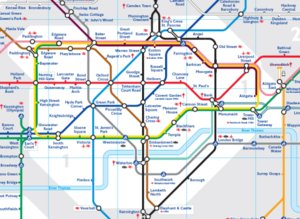
\includegraphics[height=\the\HauteurDesPhotos]{metro}\\carte du métro\end{tabular}}
\sbox{\MaBoiteAvecPhotos}{\scriptsize\begin{tabular}{c}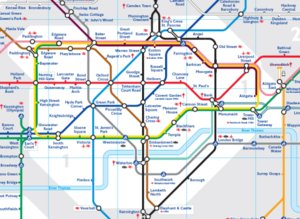
\includegraphics[height=\the\HauteurDesPhotos]{metro}\end{tabular}}
\medskip
\ImageAGauche{%
La représentation schématique généralement utilisée pour représenter un réseau de métro a été mise au point, la première fois,
en 1931 par Henry Beck,\index[aut]{Beck (Henry Charles, dit Harry), 1902-1974, Anglais}
alors dessinateur industriel de 29 ans et engagé comme intérimaire par la société du métro londonien.
Facile à comprendre et à utiliser, esthétique... il est pourtant faux à tous les égards sauf deux.\\
\indent Il n'est pas à l'échelle, donc toutes les distances sont fausses; les lignes droites reliant les stations
ne traduisent absolument pas le cheminement réel du métro sous les rues; les orientations sont fausses (une
ligne verticale ne signifie pas que le trajet s'effectue selon l'axe nord-sud).\\
\indent Le premier aspect exact est que si une station de métro est représentée au nord de la Tamise, alors il en est de même
pour la station réelle.
Le second aspect exact est la description du réseau: l'ordre des stations sur chaque ligne et les interconnexions
entre les lignes sont fidèles à la réalité. C'est d'ailleurs ce second aspect qui est finalement le seul dont les
voyageurs ont effectivement besoin.\\
\indent Notons enfin que cette illustration permet de comprendre aisément comment la notion de distance
peut être appréhendée en topologie.
}
\end{histoire}

\medskip
\section{Petit exemple amusant d'injection dans un Hilbert}
Soient~$V$ et~$H$ deux espaces de Hilbert sur~$\RR$ et~$V$ inclus dans~$H$
avec injection continue et~$V$ dense dans~$H$.
\medskip
Comme~$V$ est inclus dans~$H$, l'injection est tout bêtement \(i\colon x\mapsto x\).

\medskip
Dans ces conditions, \(H\) est un espace de Hilbert avec un produit scalaire \((\ \mid\ )_H\),
et \(V\) muni du produit scalaire induit est un sous-espace dense, donc
\textcolorred{ne peut pas être un espace de Hilbert} par restriction du produit
scalaire \((\ \mid\ )_H\).
La structure hilbertienne de \(V\) est définie par un produit scalaire \((\ \mid\ )_V\) propre à \(V\).

\medskip
Il y a donc deux topologies sur \(V\): la topologie hilbertienne propre à \(V\) et la
topologie héritée de la structure hilbertienne de \(H\).
La continuité de l'injection \(i\) impose donc une condition sur ces topologies:
la topologie hilbertienne de \(V\) est plus fine que la trace sur \(V\) de la topologie hilbertienne de \(H\).

\medskip
\textcolorgris{... et maintenant que le terme «injection» a été prononcé, il est temps
de passer au chapitre suivant...} 